\newpage
\section{Results and Evaluation}
\subsection{Experiment Setup}
The experiment is completed with a 3.1 GHz Intel Core i5 Processor with 8GB of memory.The four implemented encoding schemes was first compared using size of CNF it generated. Then the encoded results were fed into the model counter miniC2D, this model counter was selected because it's one of the newest model counting tool available and according to \cite{minic2d}, it outperforms many of the model counting tools. Number of Clauses in the CNF is used in the evaluation because it size of the CNF directly influence the model counting time. Besides, Some of the data I gained from the output of model counter is also compared including Compiling time, Compile memory, cache hitrate and model couting time.\\

Since the comparison is mainly runtime, to eliminate the variance, each model counting for a encoded bench mark was done five times and took the average. The time limit is 2 hours maximum. The runtime for Full encoding was omitted because for most of the benchmarks I used, the model counter fail to output result within reasonable amount of time.\\

In the experiments and results, I first compare the number of clauses generated by Full encoding and Simplified Full encoding to show the improvement done by encoding determinism, which was mentioned in previous section that lead to the most significant reduction in the number of clauses and compiling time. Then the size of the CNF generated by Simplified encoding, Improved encoding, and Group encoding was compared.\\


\subsection{Data}
The experiment data was mainly Grid Networks from the the Rochester University The grid networks are in size N $\times$ N, the with a deterministic ratio $R$ specifying the scale of deterministic, which means the number of nodes whose values are determined given the values of their parents. \\
\textcolor{red}{detail information here}
Table 

\begin{tabular}{c|c}
     &  \\
     & 
\end{tabular}
%\footnote{https://www.cs.rochester.edu/u/kautz/Cachet/Model_Counting_Benchmarks/index.htm}. 
The dataset is chosen because Weighted model counting method perform well on highly deterministic Bayesian Networks and the Ratio indicates the deterministic extend that help the result analysis.
\subsection{Encoding determinism}
The Simplified Full Encoding captures the determinism and simplify the encoded results compared to the Full encoding. Some of the results are shown in the Table \ref{tab:enc-determin}. The results indicate that the simplification lead to significant reduction in both number of variables and size of the CNF. Larger deterministic ratio lead to larger reduction. The average reduction for Ratio\_50, Ratio\_75 and Ratio\_90 are 48.43\%, 67.09\% and 80.06\% respectively. The the visualization of the result is given in figure \ref{fig:determinism}.
\begin{table}[]
    \centering
    \begin{tabular}{c c | c c  c c c }
        \hline
        &	&	Full enc	&	Simplified 	&	Full enc & Simplified &	Average\\
        Ratio & N	&   Var Num	&   Var Num	&	clause Num	& clause Num & 	Reduction\\
        \hline
        \hline
                &12	&	1346 	& 	614	&	 4428 	&	2126 &	\\
                &14	&	1850 	&	906	&	 6116 	&	3158 &	 \\
        Ratio 50&16	&	2434    &	1186	&	 8076 	&	4156 &	48.43\%\\
                &18	&	3098    &	1494	&	 10308 	&	5260 &	\\
                &20	&	3842 	&	1826	&	 12812 	&	6428 &	\\
        \hline
                &10	&	922	    &	266	&	3012	&	918 &	\\
                &12	&	1346	&	458	&	4428	&	1608 &	\\
       Ratio 75 &14	&	1850	&	458	&	6116	&	1614 & 67.09\%	\\
                &15	&	2132	&	635	&	7062	&	2240 &	\\
                &16	&	2434	&	738	&	8076	&	2612 &	\\
        \hline
                &10	&	922	    &	178	&	3012	&	618	& \\
                &12	&	1346	&	266	&	4428	&	944	& \\
        Ratio 90&14	&	1850	&	346	&	6116	&	1238 & 80.06\%	\\
                &15	&	2132	&	487	&	7062	&	1742 &	\\
                &16	&	2434	&	366	&	8076	&	1338 &	\\
        \hline
        \hline
    \end{tabular}
    \caption{Comparing number of clauses and numbers of variables before and after encoding determinism. N indicates the size of the Grid Network}
    \label{tab:enc-determin}
\end{table}

 
\begin{figure}[h]
\centering
\begin{subfigure}{0.32\textwidth}
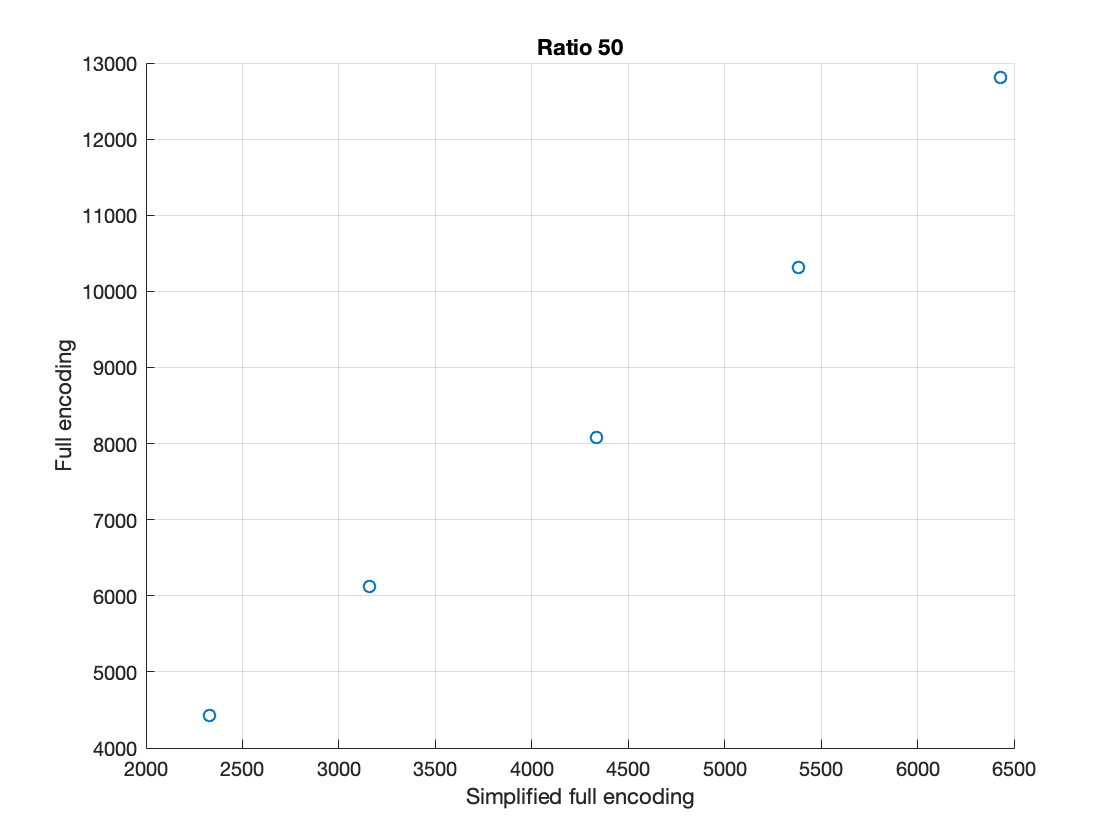
\includegraphics[width=0.9\linewidth]{pic/r50_determinism.png}
\caption{Ratio 50 determinism}
\label{fig: r50_determin}
\end{subfigure}
\begin{subfigure}{0.32\textwidth}
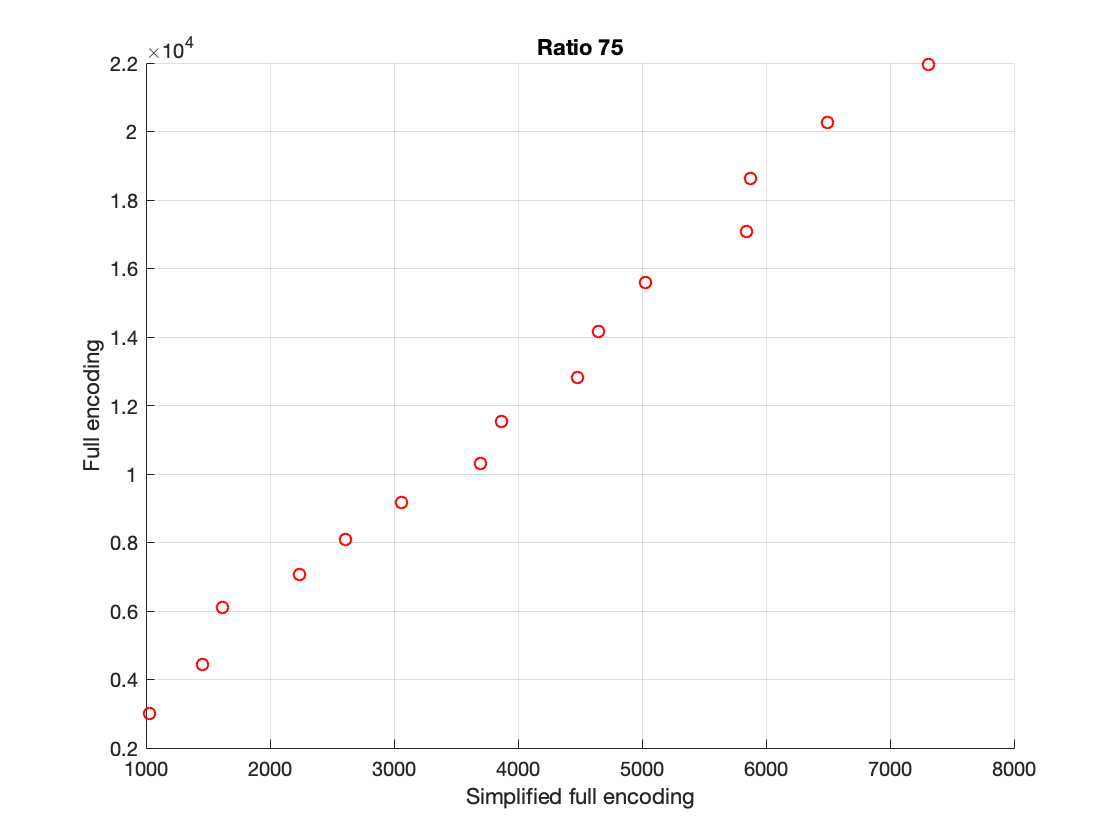
\includegraphics[width=0.9\linewidth]{pic/r75_determinism.png}
\caption{Ratio 75 determinism}
\label{fig: r75_determin}
\end{subfigure}
\begin{subfigure}{0.32\textwidth}
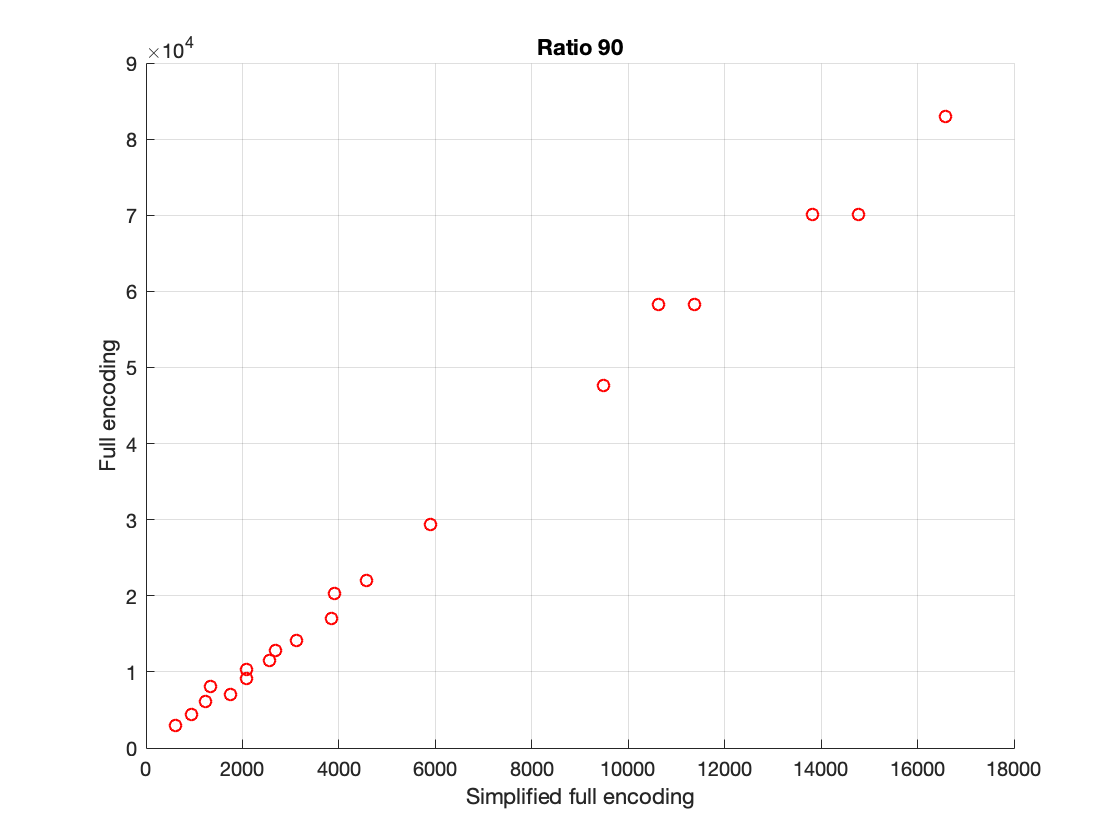
\includegraphics[width=0.9\linewidth]{pic/r90_determism.png}
\caption{Ratio 90determinism}
\label{fig: r90_determin}
\end{subfigure}
 
\caption{Full encoding vs Simplified encoding}
\label{fig:determinism}
\end{figure}

\subsection{Comparing Clause size}
Table \ref{tab:comparing the clauses} shows the group of networks three groups of networks from the repository to evaluate the three encoding schemes. Comparing the first and second row shows that with regard of size of encoded CNF file, in general Improved encoding is better than the Simplified encoding while the reduction is not that significant when comparing Improve Encoding and Group Encoding. However, despite the fact that the size is not significantly reduced, through pre-processing the CNF to make use of the semantically independent components, the model counting and compiling time as well as the file size was reduced considerably. This is discussed later in the following paragraphs.

\begin{table}[]
    \centering
    \begin{tabular}{c c c c c}
    \hline
    &	    			&	Simplified Enc	&	Improved Enc	&	Group Enc	\\
    &	Network			&	Num Clauses	&	Num Clauses	&	Num Clauses	\\
    \hline
    \hline
	&	12	-	1	&	2126	&	1052	&	976	\\
	&	14	-	2	&	3158	&	1476	&	1380	\\
Ratio 50	&	16	-	1	&	4156	&	1938	&	1804	\\
	&	18	-	3	&	5260	&	2458	&	2305	\\
	&	20	-	1	&	6428	&	3034	&	2819	\\
	\hline
	&	10	-	1	&	918	&	644	&	568	\\
	&	10	-	2	&	1048	&	662	&	594	\\
	&	10	-	3	&	1030	&	660	&	600	\\
	&	12	-	1	&	1452	&	954	&	849	\\
	&	12	-	2	&	1422	&	948	&	847	\\
Ratio 75	&	12	-	3	&	1608	&	974	&	876	\\
	&	14	-	1	&	1614	&	1252	&	1087	\\
	&	14	-	2	&	1818	&	1280	&	1131	\\
	&	14	-	3	&	1894	&	1292	&	1138	\\
	&	15	-	3	&	2240	&	1496	&	1328	\\
	&	16	-	3	&	2612	&	1714	&	1512	\\
	\hline
	&	10	-	2	&	618	&	600	&	519	\\
	&	12	-	2	&	944	&	878	&	746	\\
	&	14	-	2	&	1238	&	1196	&	1021	\\
	&	15	-	2	&	1742	&	1422	&	1243	\\
Ratio 90	&	16	-	2	&	1338	&	1528	&	1289	\\
	&	17	-	2	&	2074	&	1810	&	1571	\\
	&	18	-	2	&	2080	&	1998	&	1711	\\
	&	19	-	2	&	2552	&	2264	&	1935	\\
	&	20	-	2	&	2686	&	2492	&	2148	\\
	\hline
	\hline
    \end{tabular}
    \caption{A Comparison of number of clauses generated by Simplified encoding, Improved encoding, and Group Encoding}
    \label{tab:comparing the clauses}
\end{table}

\subsection{Model counting results}
The first analysis is based on the maximum cluster size of the tree. According to \cite{2008-literature-review}, this number is important because through exploiting topological structure for probabilistic inference run in time that is exponential in the maximum cluster size of the tree. The results showed that by encoding deterministic, weighted model counting method can successfully generate results in reasonable amount of time even the size of the cluster is large. \\
\textcolor{red}{Insert table here!!}\\

\subsection{Size of the NNF}
We then compare the file size generated in the model counter for the three encoding schemes. \\

During the model counting process, CNFs are first compiled into NNF format, and the file is stored with an .nnf extension. The compiled form support different Bayesian inference queries to be answered as many times as wanted. It has been shown in \cite{2008-literature-review} that given the same NNF, the variance of time used to answer different queries are small. So the Model counting time is used to represent the time used for bayesian inference queries.\\

Table \ref{tab:size compare} compares the size of the NNF file in MegaBytes. Comparing the second and third column, observed that in general, from Simplified full encoding to Improved Encoding, the file size increase, sometimes twice as big as the size of Simplified encoding.
This also explained the reason why model counting time is longer for Improved Encoding.
\begin{table}[]
    \centering
    \begin{tabular}{c|c c c}
    \hline
    \hline
Benchmark	&	Simp. Size (MB)	&	Impr. Size(MB)	&	Group. Size (MB)	\\
\hline
12	-	1	&	19.13	&	34.93	&	11.00	\\
12	-	2	&	30.43	&	28.30	&	10.53	\\
12	-	3	&	30.13	&	34.47	&	21.60	\\
12	-	4	&	28.80	&	52.87	&	21.83	\\
12	-	5	&	22.00	&	35.00	&	32.40	\\
14	-	2	&	43.30	&	85.63	&	31.93	\\
14	-	4	&	142.37	&	199.87	&	52.03	\\
14	-	5	&	197.93	&	315.23	&	69.23	\\
14	-	6	&	59.07	&	99.80	&	26.57	\\
14	-	7	&	319.10	&	389.10	&	173.60	\\
16	-	1	&	327.90	&	383.53	&	264.70	\\
16	-	2	&	736.83	&	1604.07	&	784.00	\\
16	-	3	&	464.43	&	1003.77	&	138.43	\\
16	-	4	&	945.03	&	1383.47	&	319.07	\\
16	-	5	&	731.33	&	705.90	&	313.10	\\
\hline
\hline
    \end{tabular}
    \caption{Comparing the size of the NNF file generated from the miniC2D model counter. The input is the encoded CNF using Simplified Full encoding, Improved encoding, and Group Encoding}
    \label{tab:size compare}
\end{table}
\textbf{Compling time and Counting time}:\\
\begin{table}[]
    \centering
    \begin{tabular}{ c | c c | c c | c c}
    \hline
    	    	&	Simp.	&		&	Impr. 	&	 &	Group	&		\\
   		Bench	&	Comp.	&	Count.	&	Comp. 	&	Count. &	Comp. 	&	Count.	\\
   		mark		&	time	&	time	&	time	&time	& time	&	time	\\
   	\hline
   	\hline
12	-	1	&	3.51	&	0.32	&	1.14	&	0.52	&	0.27	&	0.14	\\
12	-	2	&	5.05	&	0.55	&	1.14	&	0.37	&	0.28	&	0.14	\\
12	-	3	&	3.43	&	0.47	&	1.33	&	0.43	&	0.54	&	0.31	\\
12	-	4	&	2.23	&	0.46	&	1.96	&	0.68	&	0.54	&	0.28	\\
12	-	5	&	2.37	&	0.35	&	1.15	&	0.44	&	0.76	&	0.46	\\
14	-	2	&	5.48	&	0.68	&	3.43	&	1.25	&	0.90	&	0.50	\\
14	-	4	&	20.26	&	2.51	&	5.76	&	2.97	&	1.26	&	0.70	\\
14	-	5	&	109.74	&	3.70	&	8.10	&	4.39	&	1.99	&	1.05	\\
14	-	6	&	19.24	&	0.93	&	2.89	&	1.38	&	0.88	&	0.40	\\
14	-	7	&	26.50	&	5.74	&	12.27	&	5.60	&	4.25	&	2.84	\\
16	-	1	&	70.52	&	5.72	&	13.04	&	5.26	&	6.34	&	4.59	\\
16	-	2	&	75.09	&	13.49	&	52.42	&	26.44	&	33.17	&	12.07	\\
16	-	3	&	100.47	&	8.11	&	46.78	&	15.84	&	3.58	&	2.27	\\
16	-	4	&	96.44	&	16.40	&	47.56	&	22.33	&	8.52	&	3.66	\\
16	-	5	&	40.38	&	12.37	&	17.37	&	10.42	&	10.60	&	4.20	\\
	\hline
	\hline
    \end{tabular}
    \caption{A Comparison of Compiling time and Counting time with Simplified Encoding, Improved Encoding and Group Encoding Using Ratio 50 Bayesian Networks}
    \label{tab:comparing time}
\end{table}
Recall that from Simplified encoding to Improved encoding then to Group encoding, these encoding schemes tend to produce smaller CNFs. Comparing Simplified Full Encoding with Improved Encoding shows that the latter method consistently have shorter compiling time.  the extra amount of time to count models from the compiled file is much less than the time used to Compiling the CNF to NNF.\\

Comparing column 4 and column 6, the results showed that although similar number of clauses are generated, the Group encoding tends to have much shorter compliling time. It was shown in \cite{2006-enc3} that the Group encoding tend to generate clauses that have fewer occurence of irrelevant variables which benifits both the compiling time and the model counting time. For some of the benchmarks in the experiment, both Simplified encoding and Improved encoding failed to generate results in the model counter while the Group encoding managed to answer inference queries within the time limit. Some of the results are shown in Table \ref{tab:good Group encoding}\\
\begin{table}[]
\centering
\begin{tabular}{c|c c | c c | c c}
    \hline
    	&	Simpl.	&		&	Improved	&		&	Group	&		\\
    
	Bench		&	Comp. 	&	Counting 	&	Comp. 	&	Counting 	&	Comp. 	&	Counting 	\\
mark	&	Time	&	Time	&	Time	&	Time	&	Time	&	Time	\\
	\hline
	\hline
    42	-	2	&	-	&	-	& 63.1533 &	77.3533	&	10.0803	&	0.38467	\\
    42	-	3	&	-	&	-	&	-	&	-	&	118.6946	&	18.7187	\\
    42	-	4	&	-	&	-	&	-	&	-	&	60.56634	&	10.57233	\\
    42	-	5	&	-	&	-	&	-	&	-	&	255.5615	&	49.5615	\\
    \hline
\end{tabular}
\caption{Some of the bench marks when Improved encoding fail but Group encoding success}
    \label{tab:good Group encoding}
\end{table}

\subsection{When Group encoding offers no advantages}
So far, with regard the the number of clauses, compiling time and model counting time, Group encoding outperforms the other two encoding schemes we are comparing with. However, the run-time of QM algorithm is exponentially to the size of input variables. When the Bayesian network nodes have large number of parents, the QM algorithm won't be able to simplify the CNF within the time limit, thus, the whole process fail during the encoding process.

\subsection{Discussion of results}
In general, the Simplified full encoding generate the largest CNFs and have the longest model counting times, while the NNF file size after compiling the input CNF file is smaller compared to the Improved Encoding.\\

Improved encoding tends to generate smaller CNFs compared to Full encoding, and the totol time spend in the model counting phase inclduding compiling and counting tends to become shorter. While the file size might be larger and sometimes it will run out of memory. The size for a 16 $\times$ 16 Grid network with Ratio 50 determinism reached 2GB.\\

Group encoding outpeform both Simplified Full encoding and Improved encoding for the benchmarks with deterministic and small CPTs, it tends to have smaller CNF size, the shortest model counting time and small NNF file sizes. However, when it comes to Bayesian networks wit large CPTs, the time spend on QM algorithm will grow exponetially, as a result, in those cases, the Group encoding won't perform well enough.

\subsection{Drawbacks of Weighted Model Counting}
The first evaluation was the comparison between different inferencing with Variable Elimination and 

